% Constructed and checked from the problem; not a geometric proof.
\documentclass[tikz,border=8pt]{standalone}
\begin{document}
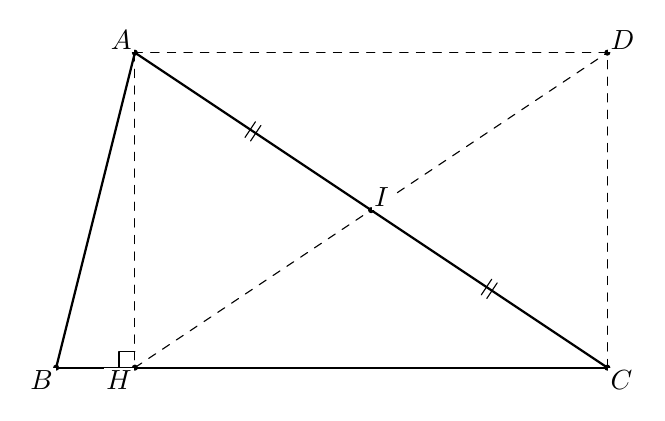
\begin{tikzpicture}[scale=1,line cap=round,line join=round]
\coordinate (p0) at (1,4);
\coordinate (p1) at (0,0);
\coordinate (p2) at (7,0);
\coordinate (p3) at (1,0);
\coordinate (p4) at (4,2);
\coordinate (p5) at (7,4);
\draw[thick] (p0) -- (p1);
\draw[thick] (p1) -- (p2);
\draw[thick] (p2) -- (p0);
\draw[dashed] (p0) -- (p3);
\draw[dashed] (p3) -- (p5);
\draw[dashed] (p3) -- (p2);
\draw[dashed] (p2) -- (p5);
\draw[dashed] (p5) -- (p0);
\draw (1,0.2023) -- (0.7977,0.2023);
\draw (0.7977,0.2023) -- (0.7977,0);
\draw (2.5313544,3.1221172) -- (2.3993358,2.9240893);
\draw (2.6006642,3.0759107) -- (2.4686456,2.8778828);
\draw (5.5313544,1.1221172) -- (5.3993358,0.9240893);
\draw (5.6006642,1.0759107) -- (5.4686456,0.8778828);
\fill (p0) circle (1.1pt) node[fill=white,inner sep=1pt,above left] {$A$};
\fill (p1) circle (1.1pt) node[fill=white,inner sep=1pt,below left] {$B$};
\fill (p2) circle (1.1pt) node[fill=white,inner sep=1pt,below right] {$C$};
\fill (p3) circle (1.1pt) node[fill=white,inner sep=1pt,below left] {$H$};
\fill (p4) circle (1.1pt) node[fill=white,inner sep=1pt,above right] {$I$};
\fill (p5) circle (1.1pt) node[fill=white,inner sep=1pt,above right] {$D$};
\end{tikzpicture}
\end{document}
